\documentclass{article}
\usepackage[T1]{fontenc}
\usepackage{tgadventor}
\usepackage{geometry}
\usepackage{titling}
\usepackage{polski}
\usepackage{graphicx}
\usepackage{float}

\renewcommand{\familydefault}{\sfdefault}

\geometry{
    top = 15mm,
    left = 25mm,
    right = 25mm,
    bottom = 25mm,
}

\begin{document}
    \begin{titlepage}
        \centering
        {\Huge\bfseries Autonomiczny robot społeczny ,,Rysiek''\par}
        
\includegraphics[width=0.5\textwidth]{figures/konar.png}\par
        {\huge Koło Naukowe Robotyków\\,,KoNaR''\par}
        {\par}\vspace{1cm}
        {\large Krzysztof Andrzejewski\par}
        {\large Wojciech Bohdan\par}
        {\large Krzysztof Kowaczek\par}
        {\large Tomasz Lubelski\par}
        {\large Michał Mastej\par}
        {\large Eryk Możdżeń\par}
        {\large Dominik Pluta\par}
        {\large Kamil Winnicki\par}
    \end{titlepage}

    \section{O projekcie}
        \subsection*{Motywacja}
            Wzrasta potrzeba technologii, które łączą funkcjonalność z empatyczną interakcją - zwłaszcza w~kontekście
            społeczeństw starzejących się, rosnącej samotności wśród młodych oraz sektorach usługowych (edukacja, opieka, rozrywka, handel).
            Rynek poszukuje rozwiązań, które nie tylko wykonują zadania, ale także budują emocjonalne więzi, redukują stres lub wspierają codzienne mikro-potrzeby
            (np. przypomnienie o lekach, inicjowanie kontaktu).
            Dodatkowo, rośnie popyt na przyjazne roboty edukacyjne dla dzieci, które uczą przez zabawę,
            oraz na automatyzację usług z elementami „osobowości” (np. hostele w gastronomii).

        \subsection*{Założenia projektowe}
            \begin{itemize}
                \item inicjowanie oraz potrzymywanie interrakcji z człowiekiem,
                \item komunikacja za pomocą kolorowych świateł i ruchów,
                \item możliwość implementacji różnych scenariuszy użycia,
                \item przyjazny \textit{design} zwierzęcia.
            \end{itemize}

        \subsection*{Cel}
            Stworzyć robota, który nie jest „narzędziem”, lecz partnerem w codziennych wyzwaniach -- od
            przpomnieniu o szklance wody, dawce leku lub zdrowej przkąsce po rozbawienie gestem.

    \section{Budowa mechaniczna}
        Realizując założenia projektowe zdecydowano się na sylwetkę rysia, głównie z powodu symptycznego usposobienia.
        Pełna konstrukcja została przedstawiona na rys. \ref{full_opisy}.
        Robot składa się z:
        \begin{itemize}
            \item smukłej ramy nośnej wraz z silnikami napędowymi (rys. \ref{frame_opisy}),
            \item pokrycia wierzchniego ze spreparowanego karonu imitującego futro,
            \item animatronicznej głowy,
            \item pojemnika/plecaka na produkty zawieszonego na czujniku tensometrycznym,
        \end{itemize}

        \begin{figure}[p]
            \centering
            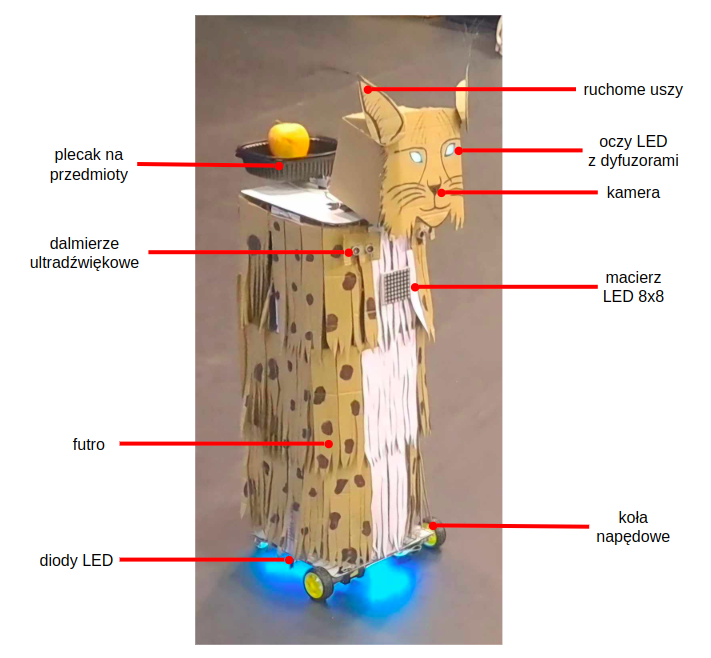
\includegraphics[width=0.75\textwidth]{figures/full_opisy.png}
            \caption{Widok robota z zewnątrz}
            \label{full_opisy}
        \end{figure}

        \begin{figure}[p]
            \centering
            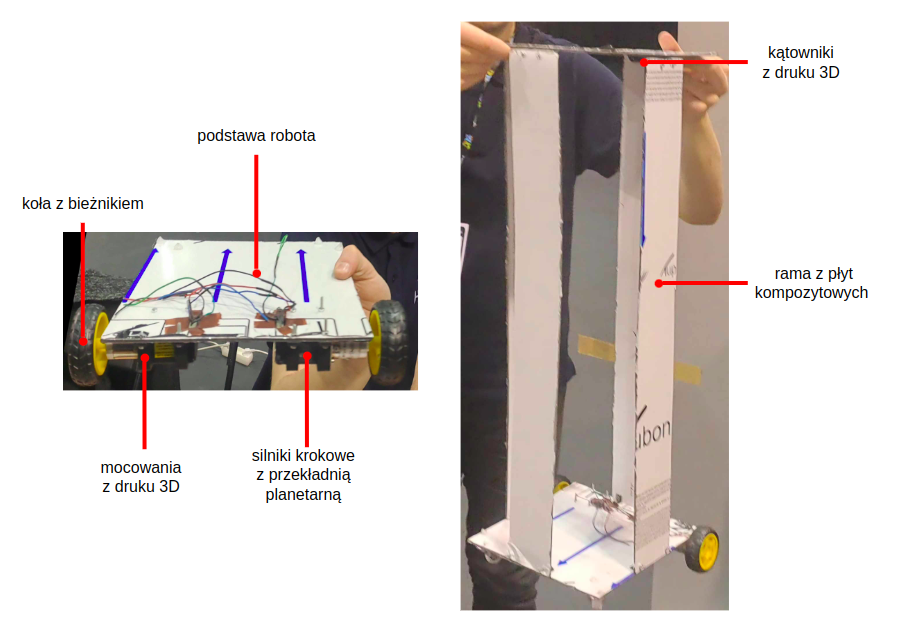
\includegraphics[width=0.85\textwidth]{figures/frame_opisy.png}
            \caption{Rama robota}
            \label{frame_opisy}
        \end{figure}

    \section{Układy elektroniki}

        \begin{figure}[p]
            \centering
            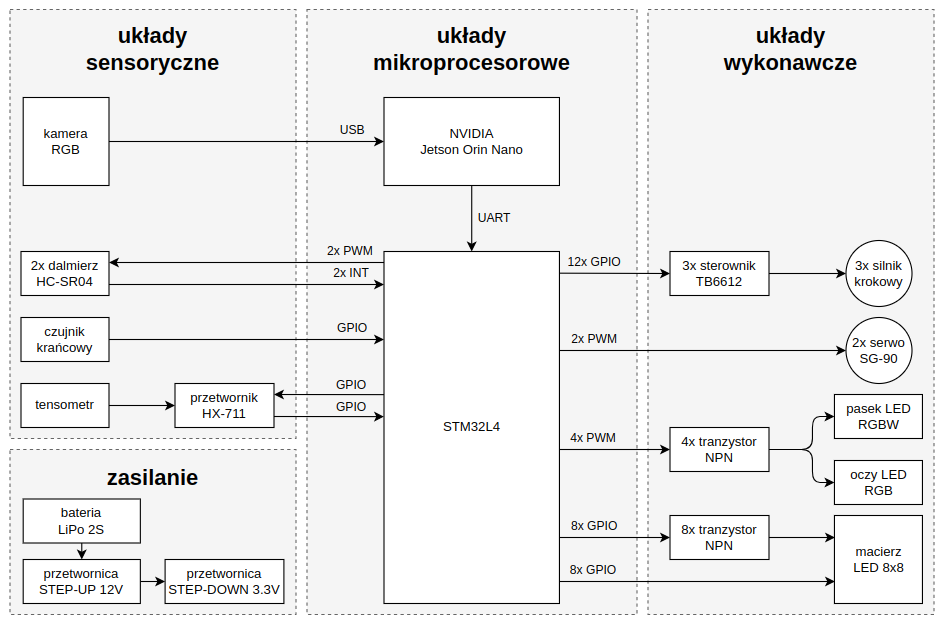
\includegraphics[width=\textwidth]{figures/elektronika_schemat.png}
            \caption{Uproszczony schemat układów elektroniki robota}
            \label{elektronika_schemat}
        \end{figure}

    \section{Oprogramowanie}

\end{document}
